\documentclass{exam}
\usepackage{mainExam}

\title{Contrôle : fonctions polynomiales du second degré}
\author{Premières Spécialité Mathématiques}
\date{27 Novembre 2024}

\begin{document}
\maketitle
\instructions{Autorisée}

\begin{questions}
\titledquestion{Etudes de pôlynomes}[8]
Pour chacune des fonctions polynomiales du second degré suivantes :
\begin{itemize}
\item Donner sa forme canonique.
\item En déduire son tableau de variation, en précisant son extremum et la valeur atteinte en cet extremum.
\item Déterminer si la fonction admet des racines, et les calculer dans ce cas.
\item En déduire son tableau de signe.
\end{itemize}
\begin{parts}
\part $p \colon x \mapsto x^2 - 6x + 9$
\part $f \colon x \mapsto -4x^2 -32x - 64$
\part $g \colon x \mapsto 3x^2 +18x + 32$
\part $h \colon x \mapsto -5x^2 + 10x - 7$
\end{parts}
\vspace*{0.5cm}
\titledquestion{Parabole}[2]
Soit $f \colon x \mapsto x^2 + bx + c$ (on remarque que $a = 1$ dans notre cas). À l'aide de la parabole $\mathcal{C}_f$ représentant $f$ donnée ci-après, en déduire la valeur de $b$ et de $c$.
\begin{center}
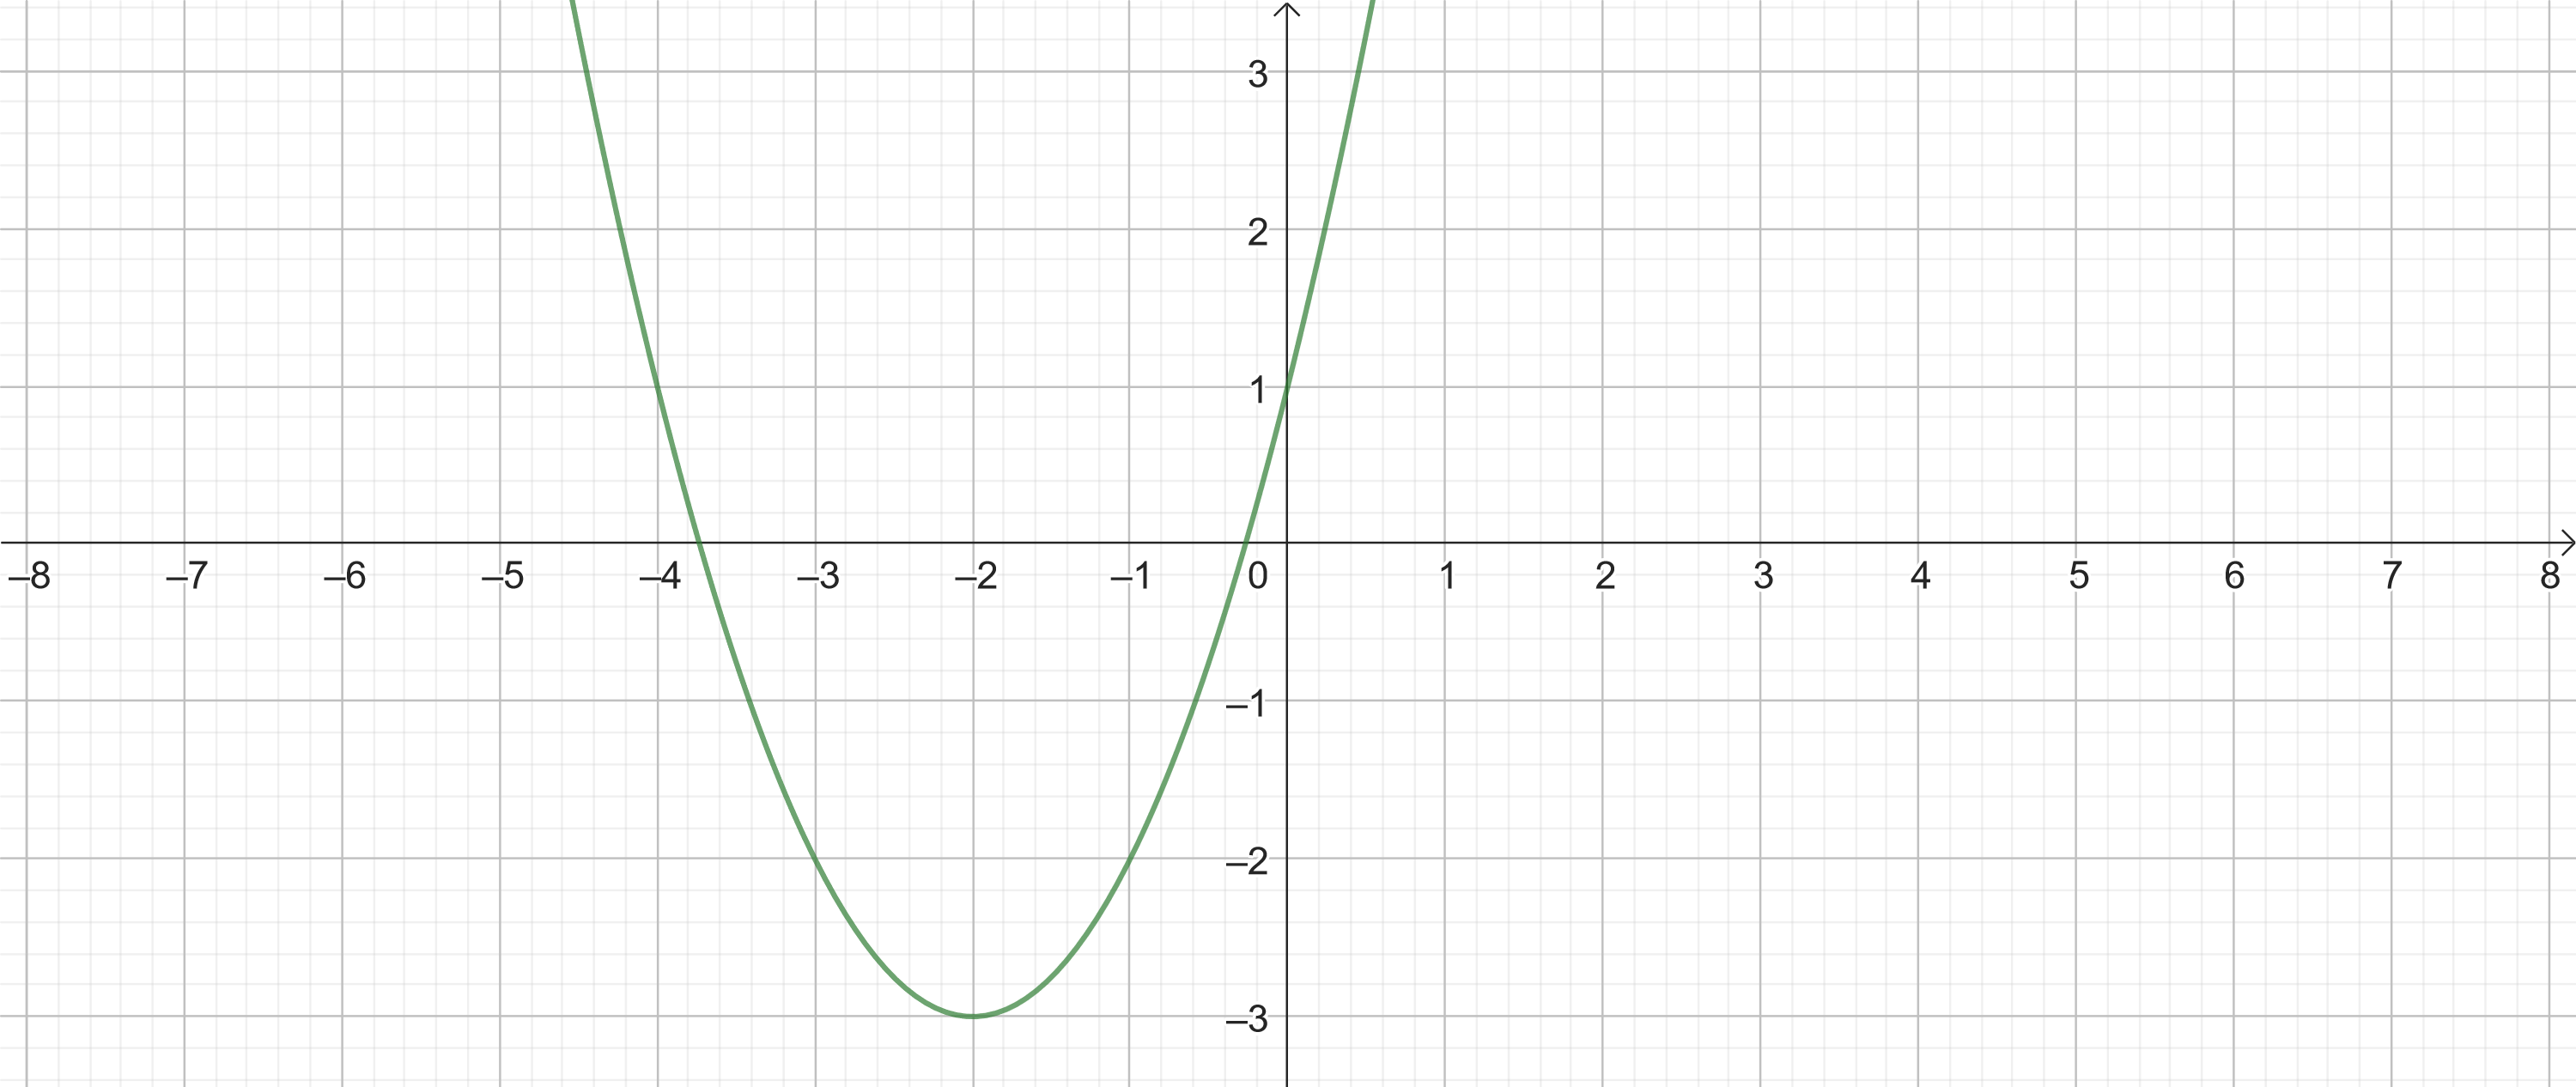
\includegraphics[width=\textwidth]{Parabole.png}
\end{center}
\newpage
\titledquestion{Drapeau}[4]
Un drapeau est donné par le motif suivant :
\begin{center}
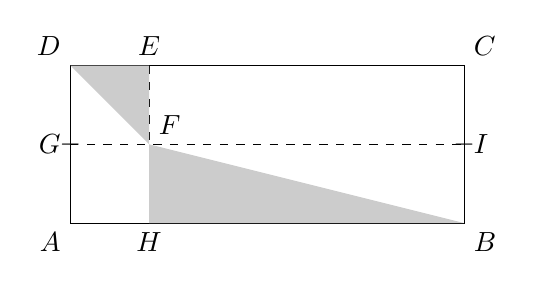
\begin{tikzpicture}
\coordinate (A) at (0,0);
\coordinate (B) at (5,0);
\coordinate (C) at (5,2);
\coordinate (D) at (0,2);
\coordinate (E) at (1,2);
\coordinate (F) at (1,1);
\coordinate (G) at (0,1);
\coordinate (I) at (5,1);
\coordinate (H) at (1,0);
\draw   
    (A) node[below left] {$A$} -- 
    (B) node[below right] {$B$} -- 
    (C) node[above right] {$C$} -- 
    (D) node[above left] {$D$} -- 
cycle;
\draw[dashed]   
    (E) node {$\shortmid$} node[above] {$E$} --
    (F) node[above right] {$F$} --
    (G) node {$-$} node[left] {$G$}
;
\draw[dashed]   
    (H) node {$\shortmid$} node[below] {$H$} --
    (F) --
    (I) node {$-$} node[right] {$I$}
;
\fill[color=gray!40] (D) -- (E) -- (F) -- cycle;
\fill[color=gray!40] (F) -- (B) -- (H) -- cycle;
\end{tikzpicture}
\end{center}
Le quadrilatère $ABCD$ est un rectangle de longueur $AB = 10$ et de largeur $BC = 5$. Le quadrilatère $DEFG$ est un carré de côté $x$, et le quadrilatère $FIBH$ est un rectangle. On note $f(x)$ l'aire de la partie grisée, c'est à dire l'aire de $DEF$ et l'aire de $FBH$.
\begin{parts}
\part Justifier que l'ensembre de définition de $f$ est $[0;5]$.
\part Justifier que l'aire grisée est donnée par
\begin{equation*}
f(x) = x^2 - 7,5x + 25
\end{equation*}
\part En déduire la valeur de $x$ pour laquelle l'aire grisée est minimale.
\part En déduire la valeur de $x$ pour laquelle l'aire grisée vaut le quart de l'aire du rectangle $ABCD$.
\end{parts}
\vspace*{0.5cm}
\titledquestion{Equation à paramètres}[4]
\begin{parts}
\part Résoudre l'équation $m^2 - 4m - 32 = 0$ sur $\R$.
\part Pour quelles valeurs de $m$ l'équation
\begin{equation*}
(m + 8)x^2 + mx + 1 = 0 
\end{equation*}
admet une unique solution dans $\R$.
\end{parts}
\vspace*{0.5cm}
\titledquestion{Radicaux imbriqués \emph{(Bonus)}}[2]
Montrer que $\sqrt{2 + \sqrt{2 + \sqrt{2 + \sqrt{\dots}}}} = 2$.

\emph{Indication : poser $X = \sqrt{2 + \sqrt{2 + \sqrt{2 + \sqrt{\dots}}}}$;  puis exprimer $X^2$ en fonction de $X$.}
\end{questions}
\end{document}